\section{Experiments}
In this part we compare RNLLS with GP and Naive method. 
\subsection{Data}
\subsubsection{Synthetic}
Synthetic datasets are created as follows. Firs using msms prgram, we created a population for $F$ founding haplotypes. Then a population of n homozygote diploid individuals are randomly created as initial population for each simulation. Given initial population, we used simuPop to perform forward simulation by randomly choosing the site under selection. Allele frequency of the populations at generations 10,20,30,40,50 are recorded, i.e. $\Tc=\{10,20,30,40,50\}$
\subsubsection{Real}

\subsection{Results}
\begin{figure}
  \centering
    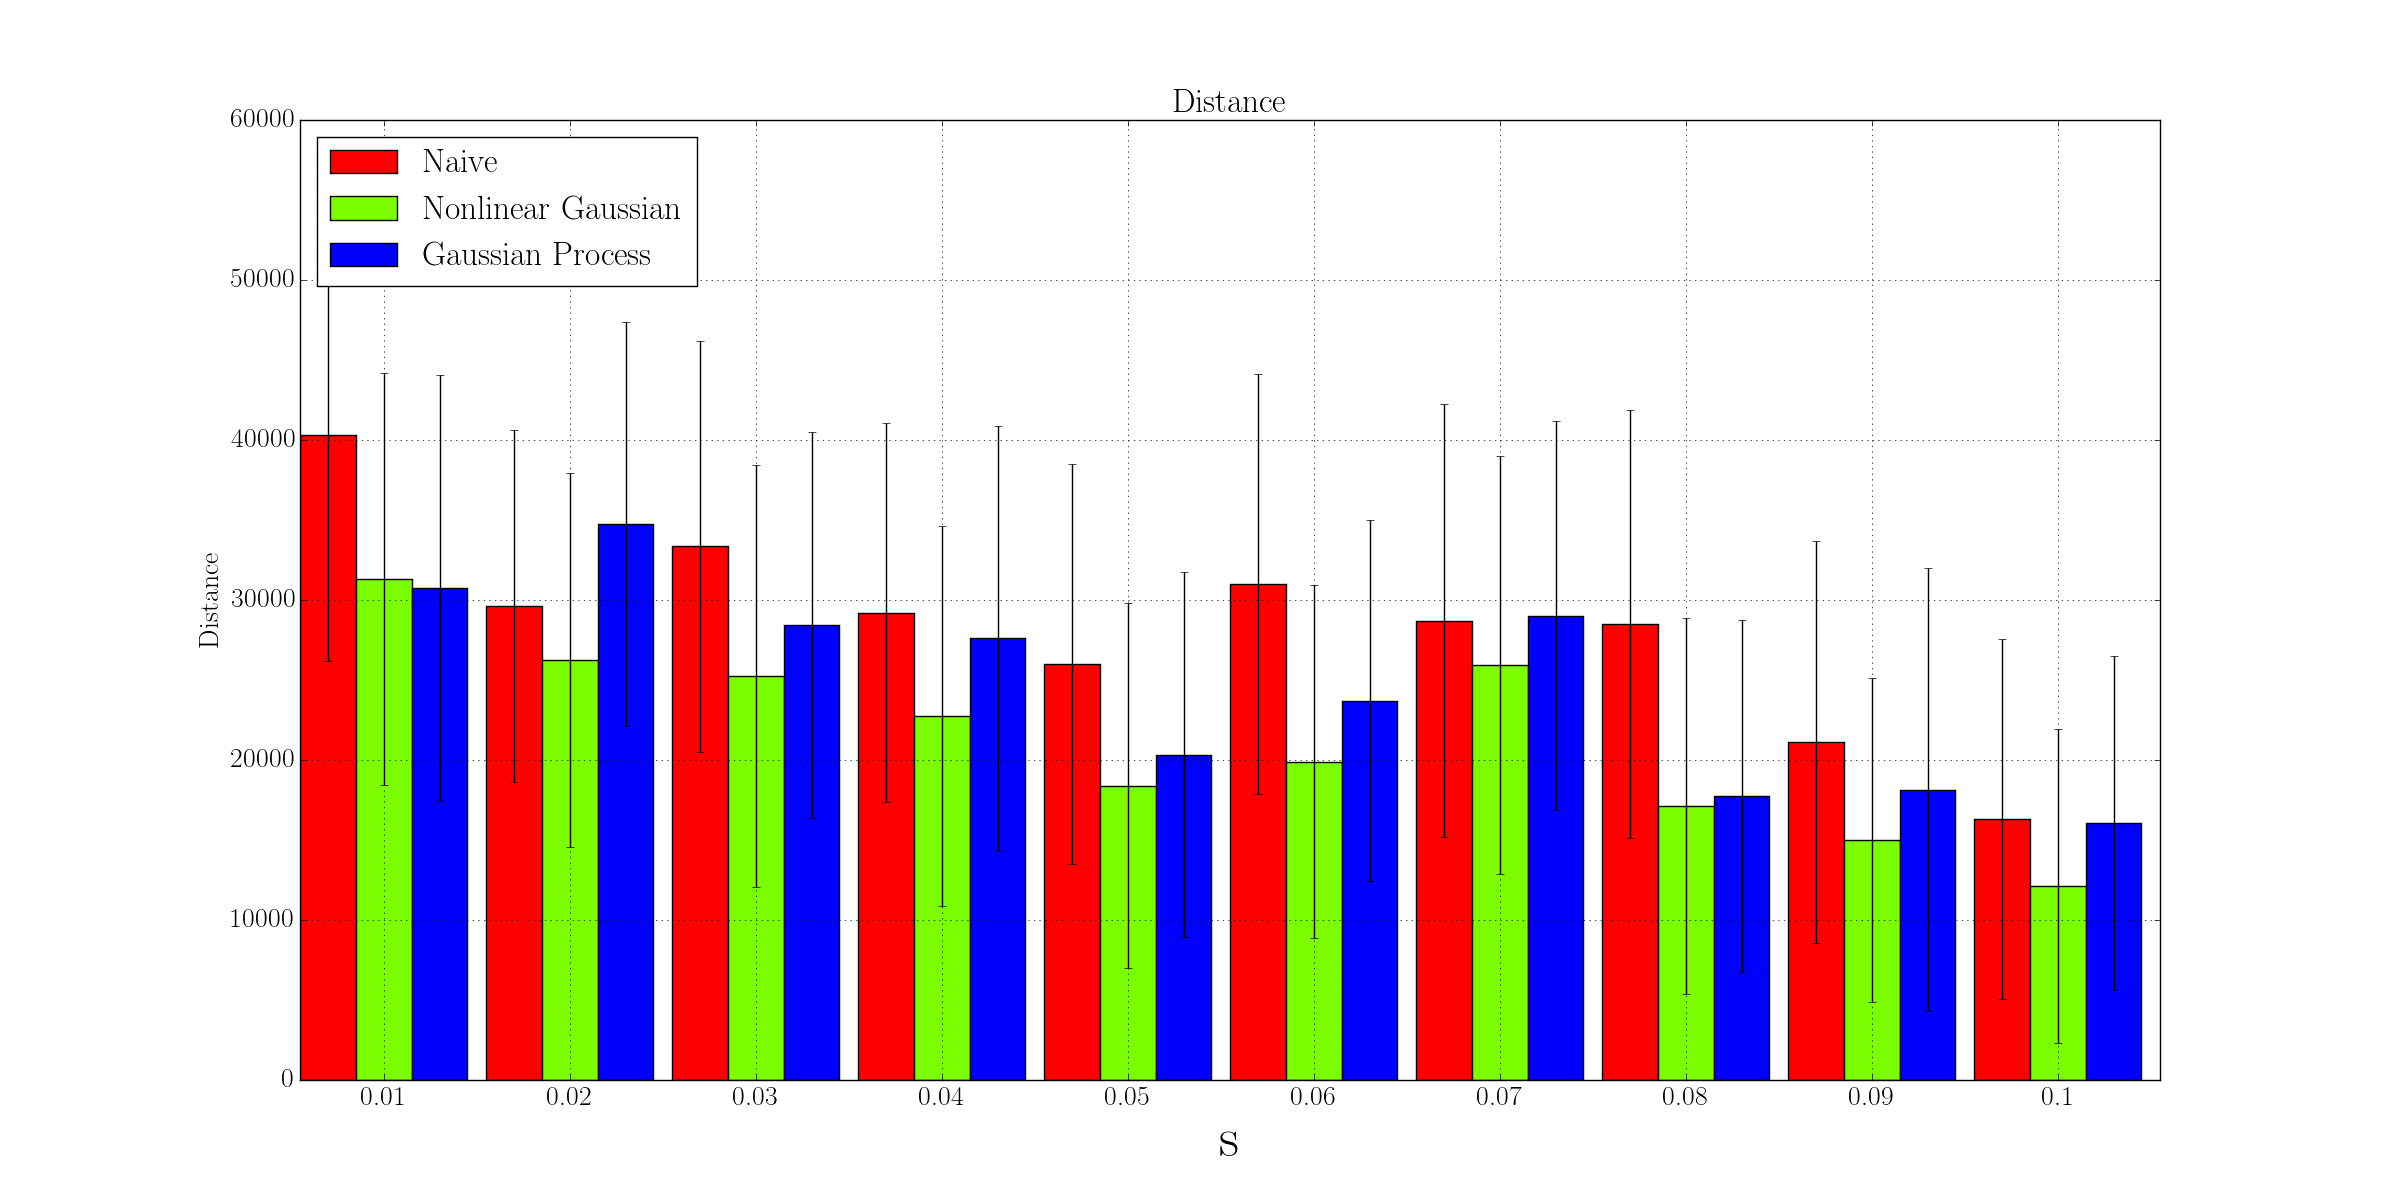
\includegraphics[width=\textwidth]{dist}
\end{figure}

\begin{figure}
  \centering
    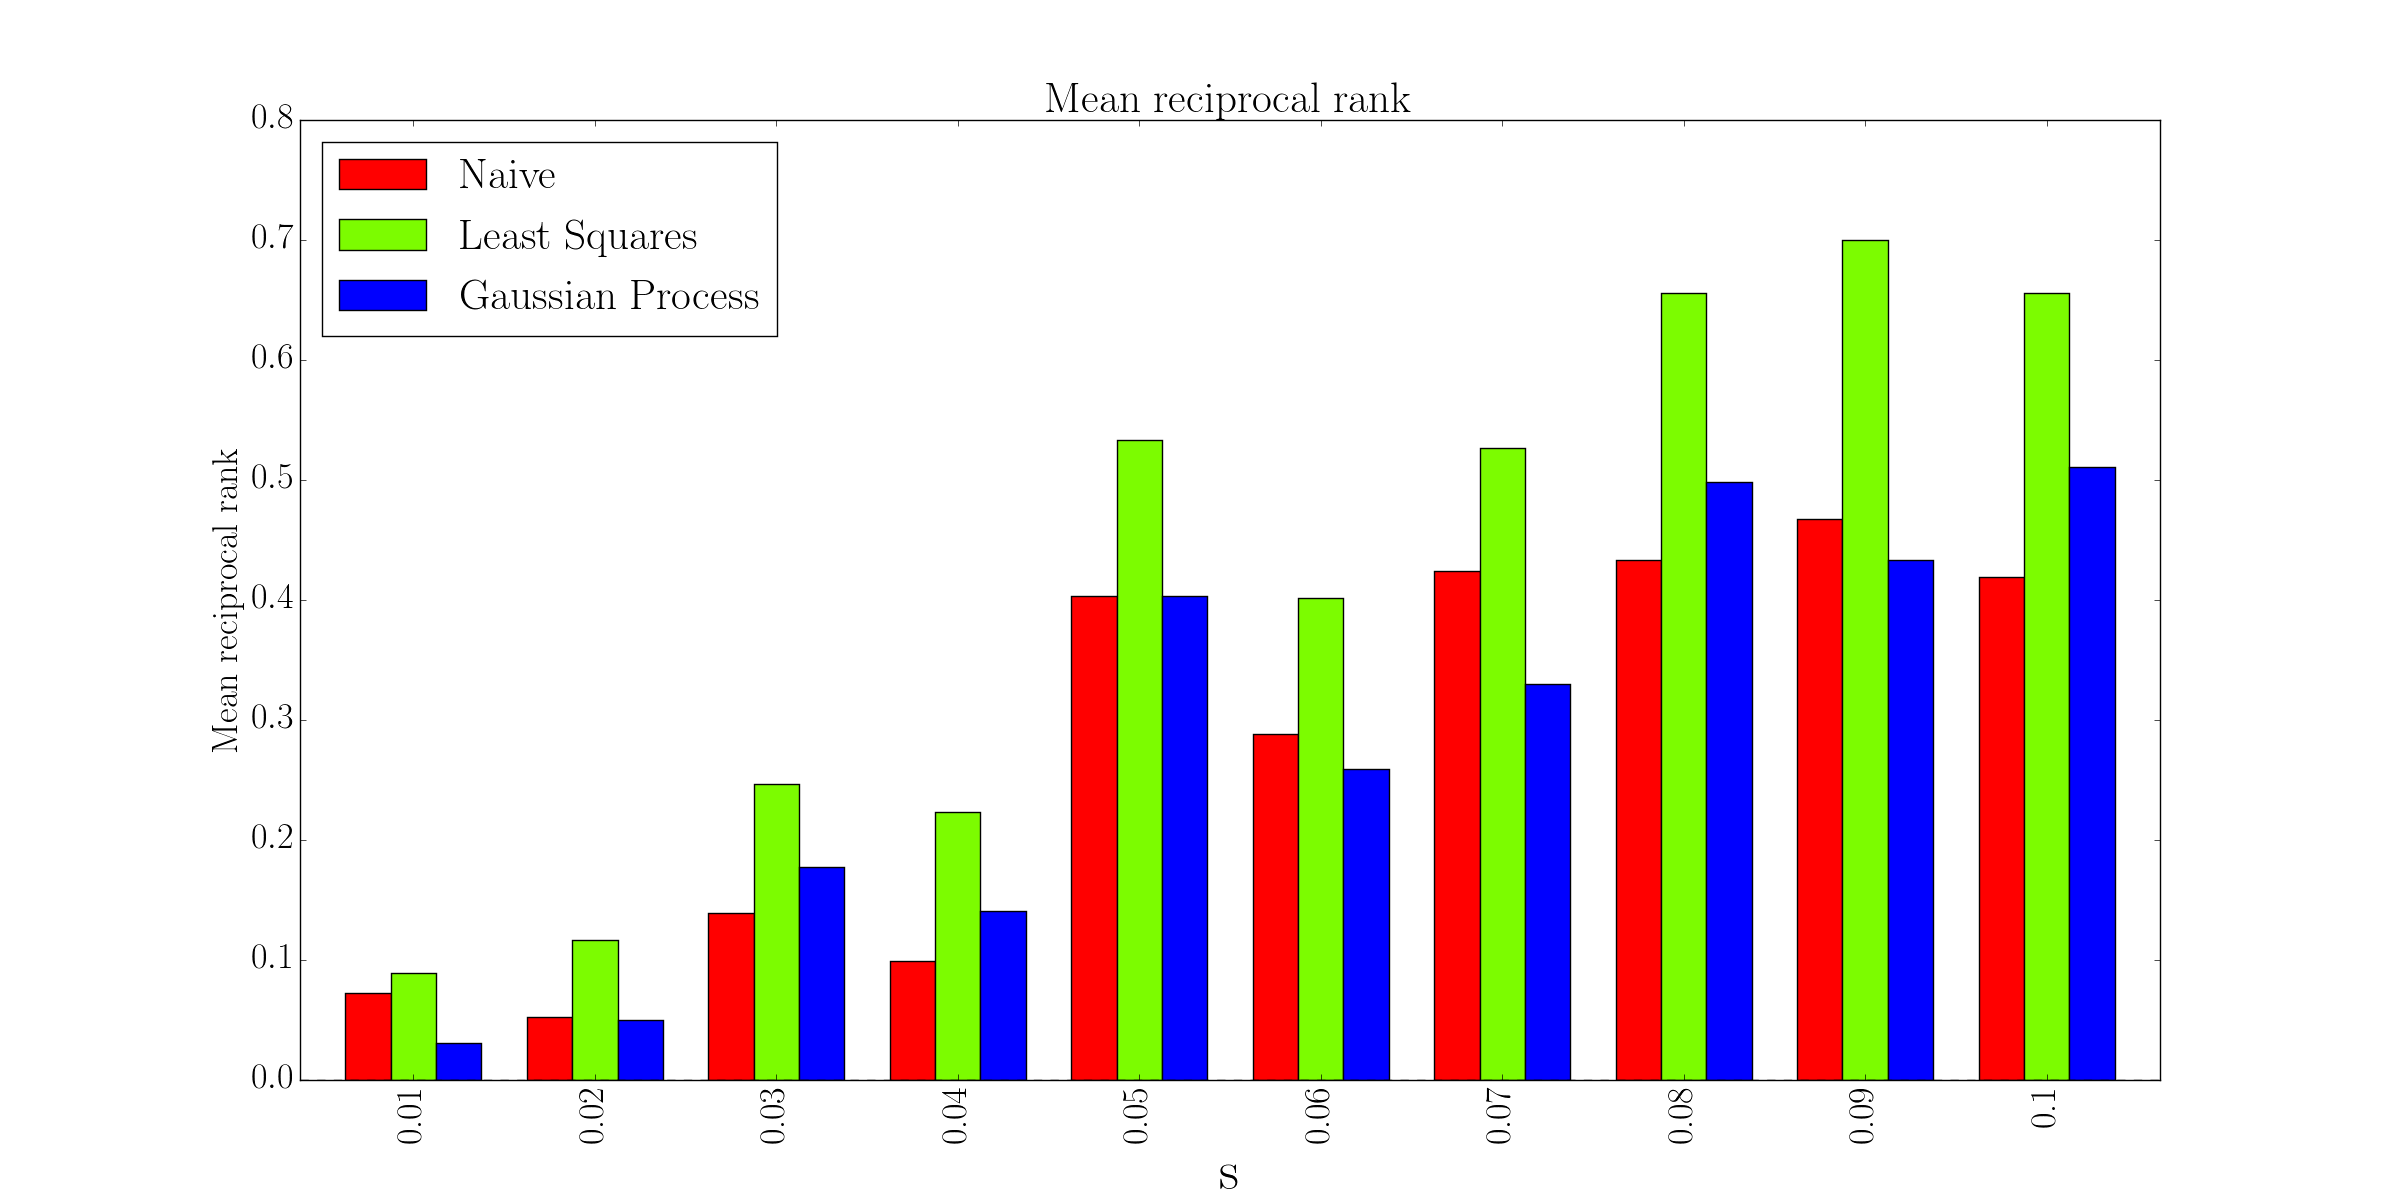
\includegraphics[width=\textwidth]{mrr}
\end{figure}

\begin{figure}
  \centering
    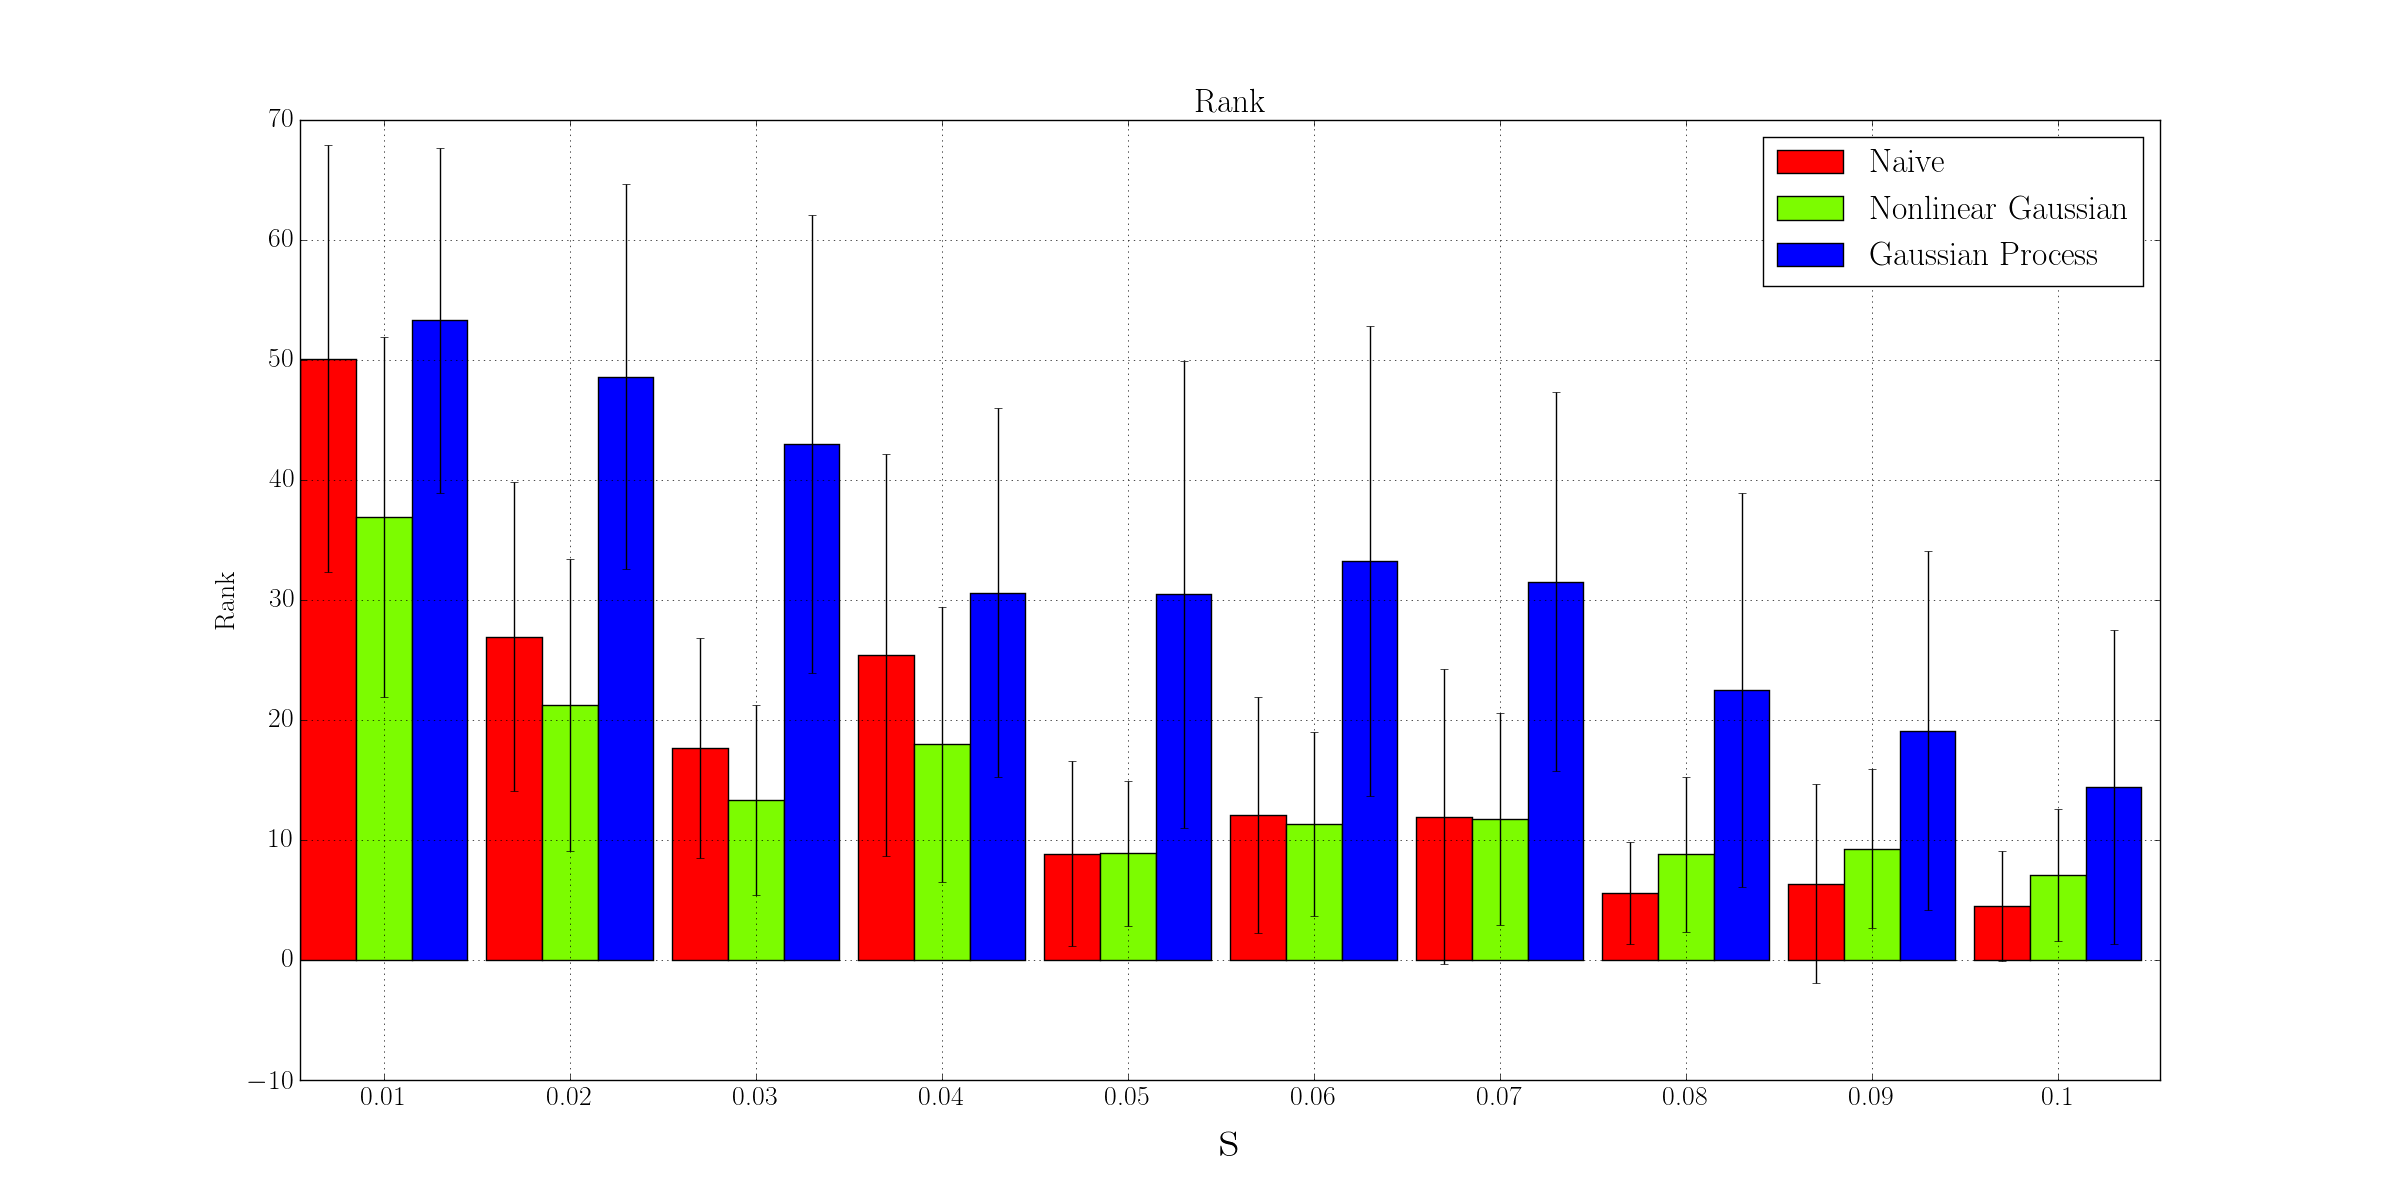
\includegraphics[width=\textwidth]{rank}
\end{figure}

\begin{figure}
  \centering
    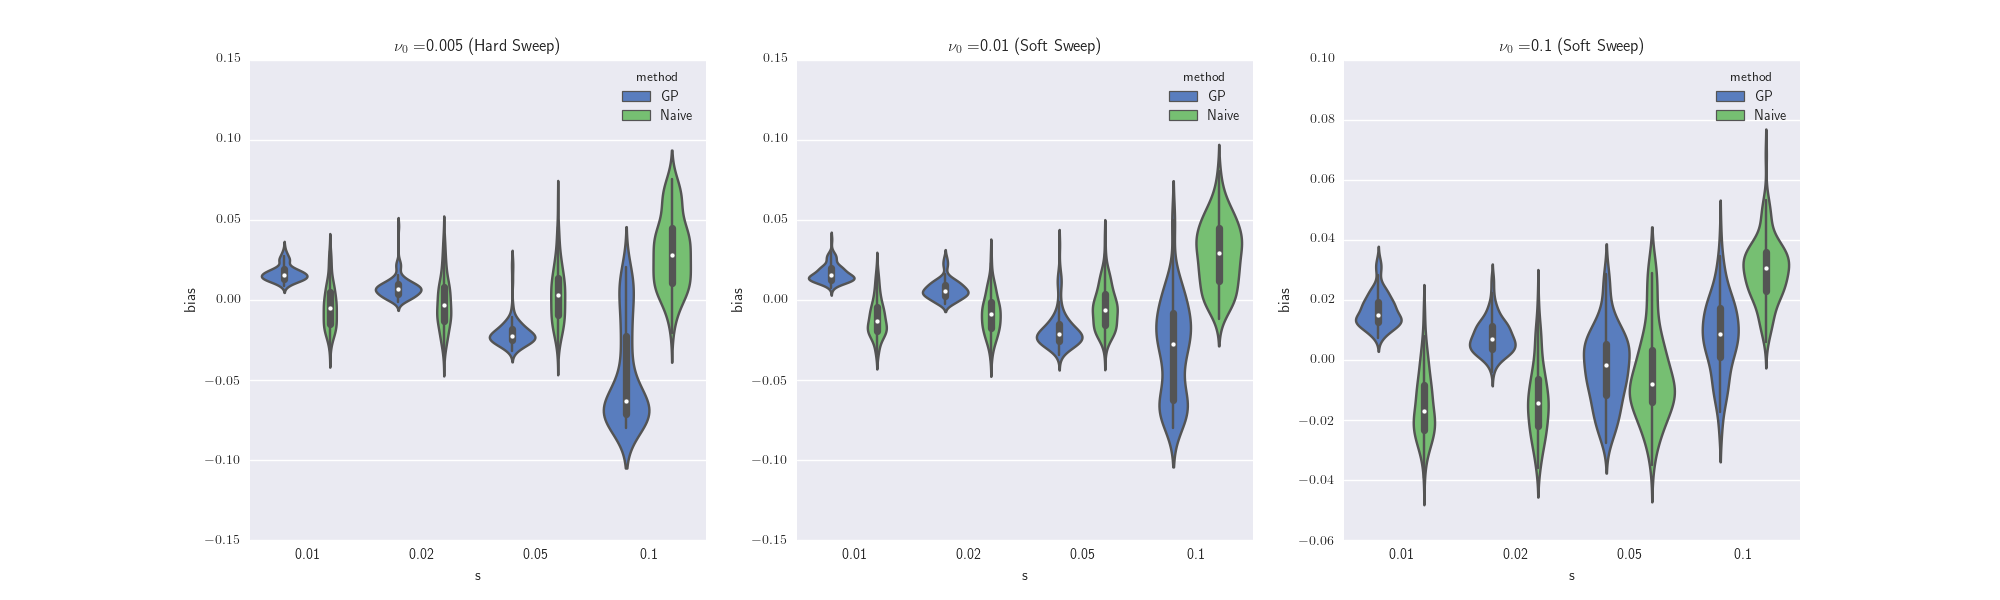
\includegraphics[width=\textwidth]{bias}
\end{figure}

\begin{figure}
  \centering
    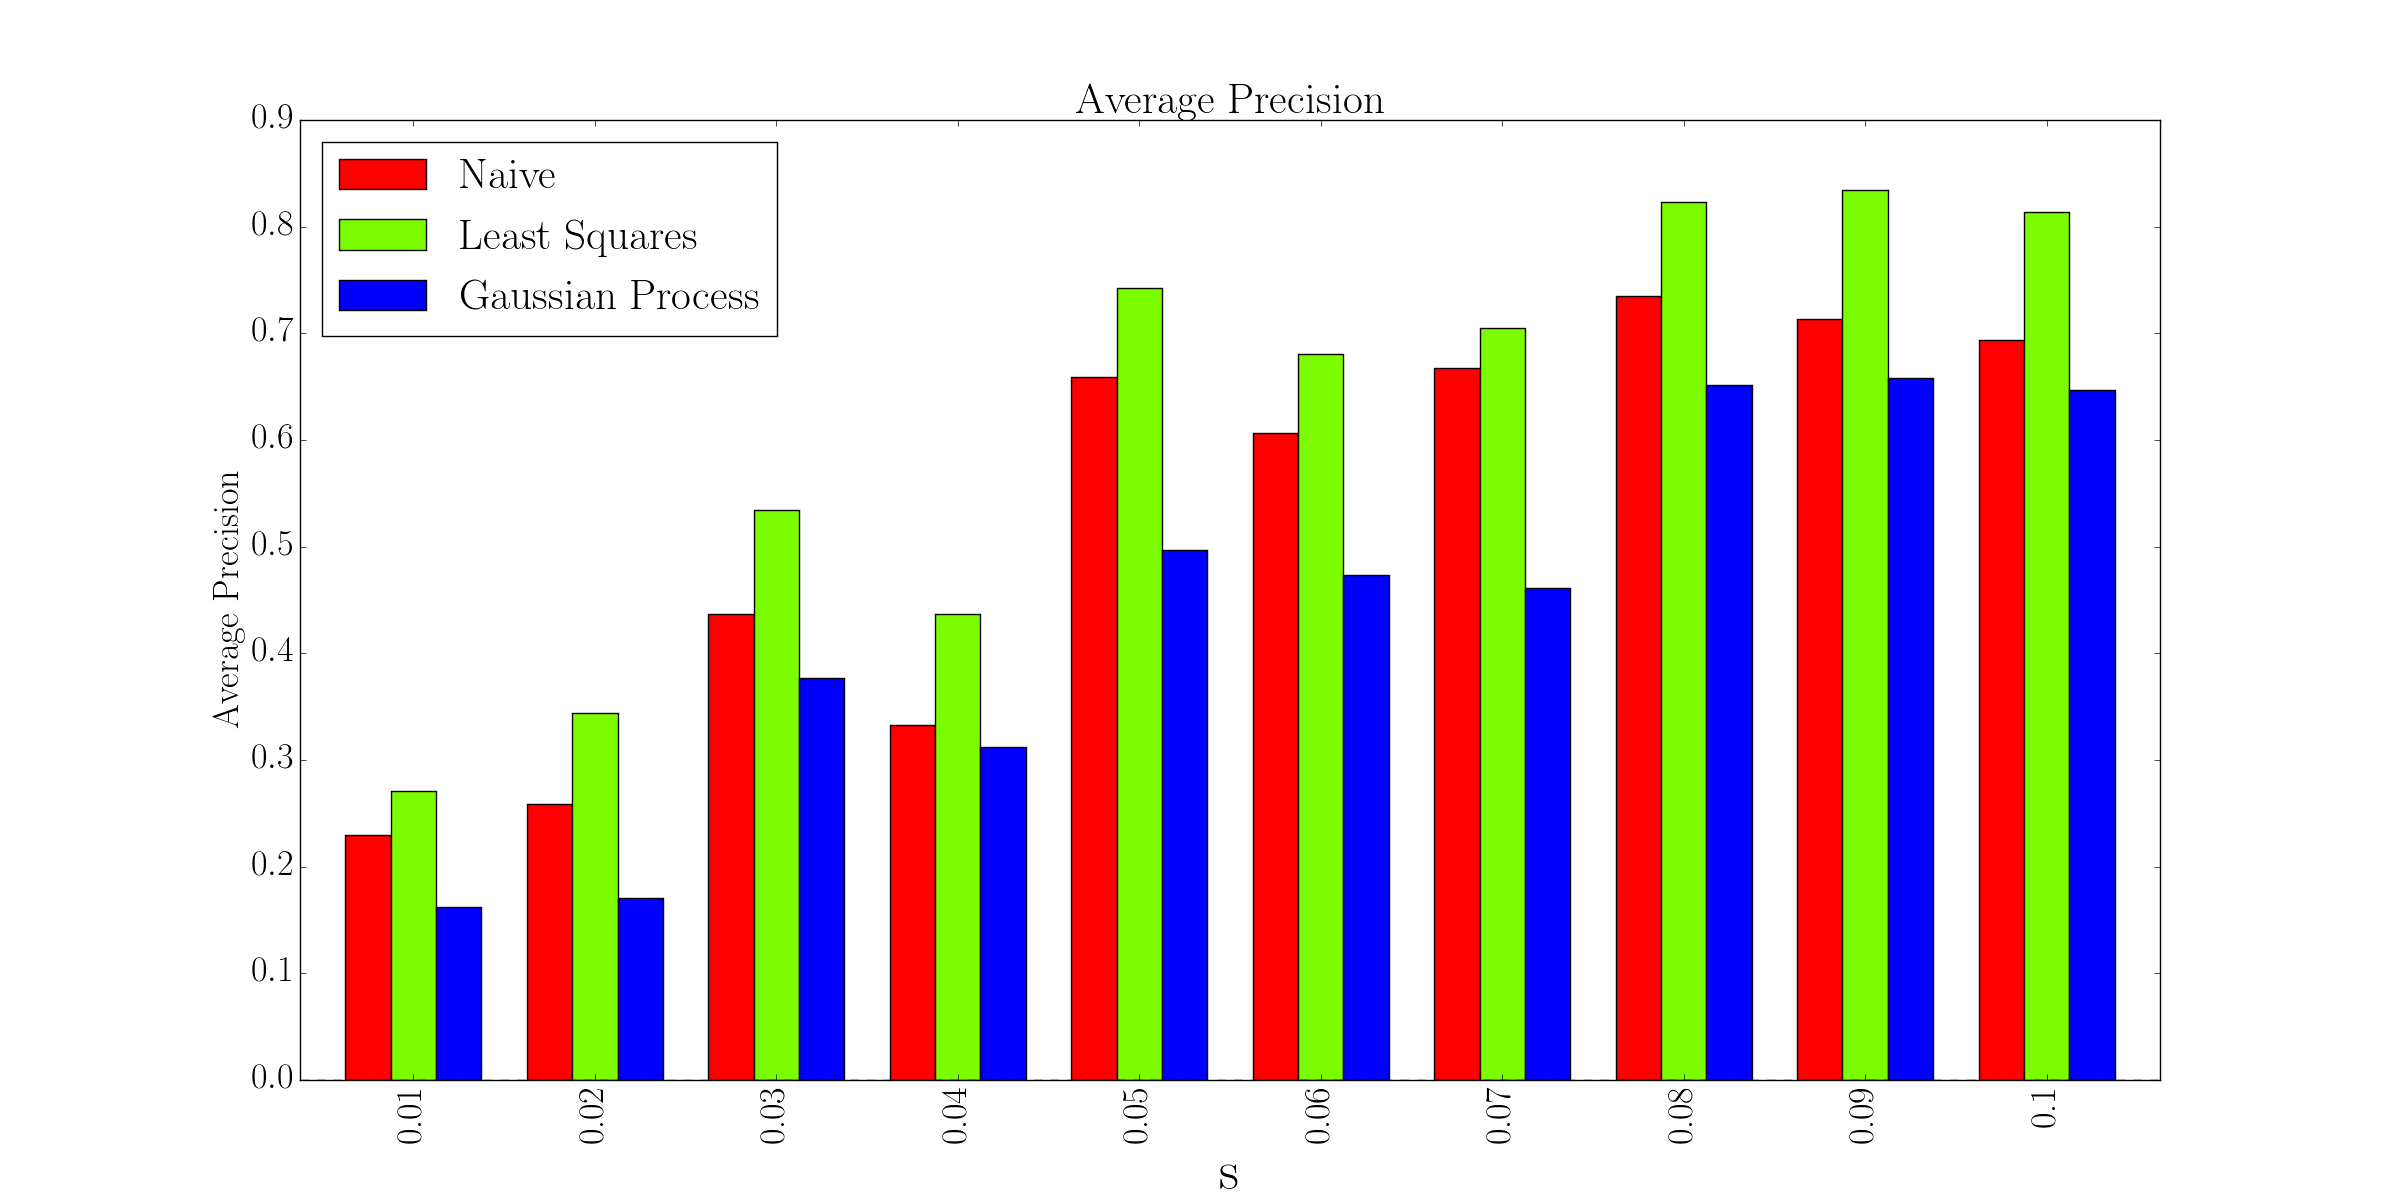
\includegraphics[width=\textwidth]{ap}
\end{figure}